%!TEX root=../GaugeCNNTheory.tex

\subsection{تبدیلات میدان کرنل و کانولوشن‌های \lr{\textit{GM}}}
\label{sec:gauge_conv_main}


عملیات اصلی شبکه‌های کانولوشنی، عملگر کانولوشن است که الگوهای مشخصه ویژگی‌ها را از یک همسایگی محلی در اطراف هر نقطه $p\in M$ به صورت خطی در یک بردار ویژگی جدید $\fout(p)$ جمع می‌کند.
یک کرنل کانولوشن گسترده فضایی، جزئیات این انباشت را تعیین می‌کند.
اصل کوواریانس نیازمند استقلال از مختصات و در نتیجه یک قانون تبدیل خاص برای کرنل‌ها تحت تبدیلات پیمانه است.
همانند مثال‌های قبلی، یک تقاضای اضافی برای اشتراک‌گذاری وزن منجر به الزامی برای کرنل الگو می‌شود تا نسبت به پیمانه هموردا ($G$-راهبر) باشد.

مطابق با بخش قبل، ما به وضوح بین الزامات استقلال از مختصات و اشتراک‌گذاری وزن تمایز قائل می‌شویم.
بنابراین، بخش~\ref{sec:kernel_field_trafos} با بحث در مورد میدان‌های کرنل و قوانین تبدیل آن‌ها بدون الزام به اینکه کرنل‌ها در موقعیت‌های جداگانه به هم مرتبط باشند، شروع می‌شود.
چنین میدان‌های کرنل نامحدودی منجر به \emph{تبدیلات میدان کرنل} می‌شوند که تبدیلات انتگرالی هستند و می‌توان آن‌ها را به عنوان پیش‌درآمدهای کانولوشن‌ها در نظر گرفت.
کانولوشن‌های واقعی $\GM$ که توسط یک کرنل الگوی مشترک و لزوماً هموردای پیمانه‌ای پارامتری می‌شوند، در بخش~\ref{sec:gauge_conv} تعریف شده‌اند.
به عنوان یک آماده‌سازی، در بخش بعدی~\ref{sec:observers_view}، نمایش‌های محلی میدان‌های ویژگی را بر روی فضاهای مماس توصیف خواهیم کرد، جایی که آن‌ها با کرنل‌های کانولوشن تطبیق داده می‌شوند.

\subsubsection{دیدگاه یک ناظر محلی به میدان‌های ویژگی}
\label{sec:observers_view}

برخلاف فضاهای اقلیدسی یا فضاهای همگن کلی‌تر مانند کره، هندسه محلی یک خمینه ریمانی کلی از نقطه‌ای به نقطه دیگر متفاوت است.
بنابراین، بلافاصله مشخص نیست که یک کرنل کانولوشن چگونه باید روی~$M$ تعریف شود و چگونه می‌توان آن را بین مکان‌های مختلف به اشتراک گذاشت.
یک راه‌حل رایج این است که کرنل را طبق معمول روی یک فضای برداری مسطح و اقلیدسی~$\R^d$ تعریف کرده و آن را به جای خود خمینه، روی فضاهای مماس به اشتراک بگذاریم؛
به بخش‌های~\ref{sec:kernel_field_trafos} و \ref{sec:gauge_conv} یا کارهای قبلی~%
\cite{masci2015geodesic,poulenard2018multi,sun2018zernet,coors2018spherenet,gaugeIco2019,Wiersma2020,deHaan2020meshCNNs,Yang2020parallelFrameCNN} مراجعه کنید.
سپس، کرنل را می‌توان از طریق نگاشت نمایی ریمانی به روی خمینه نگاشت.
می‌توان آن را به گونه‌ای تصور کرد که توسط یک ناظر محلی اعمال می‌شود که ویژگی‌ها را در محیط اطراف خود نسبت به چارچوب مرجع محلی خود اندازه‌گیری می‌کند.
در این بخش به طور خلاصه به چگونگی درک میدان‌های ویژگی از دیدگاه ناظران محلی مختلف خواهیم پرداخت.
از نظر ریاضی، این موضوع به عنوان پس‌کِش (\lr{pullback}) و انتقال موازی میدان ویژگی به فضاهای مماس فرمول‌بندی می‌شود؛ برای تجسم به شکل~\ref{fig:pullback_field_exp_TpM} مراجعه کنید.

برای نگاشت بین فضاهای مماس و خمینه، ما \emph{نگاشت نمایی ریمانی} (مرتبط با اتصال لوی-چیویتا) را در نظر می‌گیریم.%
\footnote{
	حتی مدل‌هایی که یک \emph{اتصال جایگزین (سازگار با $G$) برای انتقال ویژگی‌ها} فرض می‌کنند، معمولاً از \emph{اتصال کانونی لوی-چیویتا برای محاسبه ژئودزیک‌ها} و نگاشت‌های نمایی استفاده می‌کنند.
}
با فرض اینکه خمینه برای سادگی \emph{کامل از نظر ژئودزیکی} باشد%
\footnote{
	فرض \emph{کامل بودن ژئودزیکی} $M$ به این معناست که نگاشت‌های نمایی $\exp_p$ برای هر $p \in M$ روی کل فضای مماس $\TpM$ تعریف شده‌اند.
	در مواردی که این فرض برقرار نباشد، می‌توان به \emph{پر کردن با صفر} متوسل شد، که معمولاً در شبکه‌های کانولوشنی برای تصاویر با تکیه‌گاه متناهی استفاده می‌شود.
},
نگاشت نمایی در یک نقطه خاص~$p\in M$ نگاشتی است به صورت
\begin{align}
	\exp_p: \TpM \to M \,.
\end{align}
این نگاشت، بردارهای $v\in \TpM$ را با نقاطی $\exp_p(v) \in M$ یکی می‌داند که با دنبال کردن ژئودزیک گذرنده از~$p$ با سرعت اولیه~$v$ برای یک واحد زمان به دست می‌آیند.
نگاشت نمایی با اینکه فواصل شعاعی را حفظ می‌کند، به طور کلی زوایا را تغییر می‌دهد و یک‌به‌یک نیست.
به عنوان مثال، اگر خمینه یک کره باشد، نگاشت‌های نمایی فضای مماس مربوطه را بی‌نهایت بار دور آن می‌پیچند.
با این حال، تضمین می‌شود که نگاشت نمایی یک دیفئومورفیسم محلی است اگر دامنه آن به فواصلی کوتاه‌تر از فاصله تا مکان بُرش (جایی که یک‌به‌یک بودن از دست می‌رود) محدود شود.

با داشتن نگاشت‌های نمایی، می‌توان میدان‌های ویژگی روی خمینه را به فضاهای مماس پس‌کِش کرد.
به طور خاص، اگر~$f$ یک میدان ویژگی روی~$M$ باشد، \emph{پس‌کِش} $\exp_p^*f := f \circ \exp_p$ به عنوان نگاشتی تعریف می‌شود که بردار ویژگی $f(\exp_p(v))$ از $\exp_p(v)$ را به $v\in \TpM$ نسبت می‌دهد.
توجه داشته باشید که به دلیل عدم یک‌به‌یک بودن نگاشت نمایی، هر بردار ویژگی ممکن است به چندین بردار مماس $v_1$ و $v_2$ اختصاص یابد اگر $\exp_p(v_1) = \exp_p(v_2)$ باشد ـ این پدیده تا حدودی شبیه به اثرات عدسی گرانشی در فیزیک است.
در صورتی که نگاشت نمایی یک‌به‌یک باشد، یا زمانی که آن را به شعاع یک‌به‌یک بودن آن محدود کنیم، پس‌کِش معادل بیان میدان‌های ویژگی در \emph{مختصات نرمال ژئودزیکی} است~\cite{masci2015geodesic}.

به یاد بیاورید که هدف از پس‌کِش بردارهای ویژگی به فضاهای مماس این است که بتوان آن‌ها را توسط یک کرنل کانولوشن جمع‌آوری کرد.
متأسفانه، این کار بلافاصله امکان‌پذیر نیست زیرا بردارهای ویژگی در مکان‌های مختلف در فضاهای برداری متفاوتی قرار دارند و نسبت به پیمانه‌های متفاوتی بیان می‌شوند.%
\footnote{
	یک وضعیت بسیار مشابه، تعریف مشتقات کوواریانت را انگیزه‌مند می‌کند، که آن نیز نیاز به ترکیب اشیاء هندسی دارد که در فضاهای متفاوتی زندگی می‌کنند.
}
بنابراین لازم است تمام بردارهای ویژگی $[\exp_p^*f](v)$ در یک فضای برداری و نسبت به یک پیمانه یکسان بیان شوند.
یک ایده طبیعی که توسط پولنارد و همکاران~\cite{poulenard2018multi} پیشنهاد شد، انجام این کار با \emph{انتقال موازی} بردارهای ویژگی در امتداد ژئودزیک‌هایی است که نگاشت نمایی را از $\exp_p(v)$ به~$v$ تعریف می‌کنند.%
\footnote{
	انتقال موازی در امتداد هر مسیر دیگری نیز به همان اندازه معتبر خواهد بود.
}
ما این پس‌کِش~$f$ را با انتقال اضافی با $\Expspf$ نشان می‌دهیم تا بر ارتباط نزدیک آن با پس‌کِش معمولی $\exp_p^*f$ به $\TpM$ تأکید کنیم.
شکل~\ref{fig:pullback_field_exp_TpM} یک ایده بصری از این \emph{پس‌کِش انتقال‌دهنده} میدان‌های ویژگی به فضای مماس و نمایش‌های آن $\big[\Expspf\big]^A$ و $\big[\Expspf\big]^B$ روی $\R^d$ نسبت به مختصات‌دهی‌های مختلف ارائه می‌دهد.

\begin{figure}[H]
	\centering
	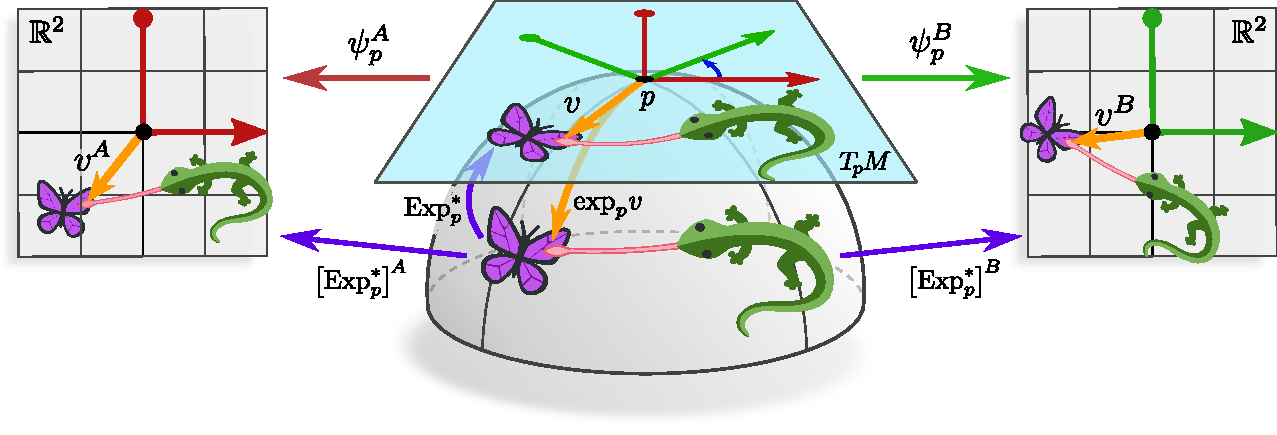
\includegraphics[width=\textwidth]{figures/pullback_field_exp_TpM.pdf}
	\caption{\small
		یک میدان ویژگی $f$ روی $M$ و نمایش محلی آن $\Expspf$ روی $\TpM$ از طریق \emph{پس‌کِش انتقال‌دهنده} $\Expsp$.
		درست مانند پس‌کِش معمولی $\exp_p^*f$ از~$f$ در امتداد نگاشت نمایی $\exp_p: \TpM \to M$، پس‌کِش انتقال‌دهنده بردارهای ویژگی $f(\exp_p(v))$ را به بردارهای مماس $v\in\TpM$ نسبت می‌دهد.
		با این حال، از آنجایی که هدف ما انباشت ویژگی‌های پس‌کِش شده با استفاده از یک کرنل کانولوشن است، آن‌ها باید در یک فضای یکسان و نسبت به یک پیمانه یکسان در~$p$ داده شوند.
		بنابراین، پس‌کِش انتقال‌دهنده علاوه بر این، انتقال‌دهنده موازی (سازگار با $G$) را در امتداد ژئودزیک از $\exp_p(v)$ به~$p$ اعمال می‌کند.
		از طریق یک پیمانه $\psi_p^X$، پس‌کِش انتقال‌دهنده $f$ روی $\TpM$ را می‌توان روی $\R^d$ به صورت $[\Expspf]^X: \R^d \to \R^c$ بیان کرد -- انتخاب‌های مختلف چارچوب‌های مرجع (ناظران) در اینجا با تغییر شکل‌های خطی مختلف میدان ویژگی مطابقت دارد.
		تبدیلات میدان کرنل و کانولوشن‌های $\GM$ یک ویژگی خروجی~$\fout(p)$ را در~$p$ با تطبیق یک کرنل~$\Kp$ روی $\TpM$ با $\Expspf$ محاسبه می‌کنند (یعنی انتگرال حاصلضرب آن‌ها را روی فضای مماس می‌گیرند؛ به معادله~\eqref{eq:kft_coord_expression} مراجعه کنید).
		{ \\
			\color{gray}
			\scriptsize
			(مارمولک‌ها و پروانه‌ها با مجوز \href{https://github.com/twitter/twemoji/blob/gh-pages/LICENSE-GRAPHICS}{\lr{\underline{Creative Commons Attribution 4.0 International}}} از توییتر اقتباس شده‌اند.)
		}
	}
	\label{fig:pullback_field_exp_TpM}
\end{figure}

ما $\Expspf$ را با تعریف آن بر حسب عبارت مختصاتی‌اش نسبت به یک انتخاب پیمانه فرمول‌بندی می‌کنیم.
برای این منظور، فرض کنید $\psi_p^A$ یک پیمانه در $p$ باشد که ویژگی‌های منتقل‌شده نهایتاً نسبت به آن بیان می‌شوند و $\psi_{\exp_p(v)}^{\widetilde{A}}$ یک پیمانه دلخواه در $\exp_p(v)$ باشد که بردار ویژگی در آن مکان را با یک بردار ضریب $f^{\widetilde{A}}(\exp_p(v)) \in \R^c$ نشان می‌دهد.
فرض کنید
\begin{align}
	\rho \big( g^{A\widetilde{A}}_{p\leftarrow\exp_p\!v} \big)
\end{align}
انتقال‌دهنده موازی سازگار با $G$ برای ضرایب بردار ویژگی در امتداد ژئودزیک از $\exp_p(v)$ به~$p$ باشد.
سپس ما \emph{پس‌کِش انتقال‌دهنده} را در مختصات به صورت زیر تعریف می‌کنیم
\begin{align}\label{eq:transporter_pullback_in_coords}
	\big[\mkern-2mu \Expspf \big]^A:\ \R^d \to \R^c,\quad v^A &\mapsto\ \big[\mkern-2mu \Expspf \big]^A (v^A)
	\notag \\[1.5ex]
	& \,:=\ 
	\rho\pig( g^{A\widetilde{A}}_{p \,\leftarrow\, \exp_p (\psi_p^A)^{\shortminus1}(v^A)} \pig) \cdot
	f^{\widetilde{A}} \pig( \exp_p \big(\psi_p^A\big)^{\mkern-2mu-1}(v^A) \pig) \,,
\end{align}
که در آن $v = \big(\psi_p^A\big)^{-1} (v^A) \in \TpM$ بردار مماس بدون مختصات است که توسط ضرایب $v^A$ از طریق~$\psi_p^A$ به آن ارجاع داده می‌شود.
همانطور که قبلاً ادعا شد، انتخاب پیمانه $\psi_{\exp_p(v)}^{\widetilde{A}}$ در $\exp_p(v)$ به دلیل استقلال مختصاتی تمام معادلات، بی‌ربط است و حذف می‌شود.
به طور خاص، می‌توانستیم از هر پیمانه دیگری مانند $\psi_{\exp_p(v)}^{\widetilde{B}}$ در $\exp_p(v)$ استفاده کنیم، که منجر به تبدیلات پیمانه
$
\rho\big( g^{A\widetilde{B}}_{p \,\leftarrow\, \exp_p(v)} \big)
= \rho\big( g^{A\widetilde{A}}_{p \,\leftarrow\, \exp_p(v)} \big)
\rho\big( g_{\exp_p(v)}^{\widetilde{B}\widetilde{A}} \big)^{-1}
$
برای انتقال‌دهنده طبق معادله~\eqref{eq:transporter_gauge_trafo} و
$
f^{\widetilde{B}} \big( \exp_p(v) \big)
= \rho\big( g_{\exp_p(v)}^{\widetilde{B}\widetilde{A}} \big)
f^{\widetilde{A}} \big( \exp_p(v) \big)
$
برای ضرایب بردار ویژگی طبق معادله~\eqref{eq:gauge_trafo_features} می‌شود، که هنگام ترکیب هر دو عبارت، یکدیگر را خنثی می‌کنند.

با این حال، پس‌کِش انتقال‌دهنده $[\Expspf]^A$ همچنان به پیمانه در $p$ بستگی دارد و بنابراین تحت تبدیلات پیمانه $g_p^{BA}$ در~$p$ تبدیل می‌شود.
مانند هر تابع مختصاتی، قانون تبدیل آن توسط تبدیلات پیمانه بر روی دامنه~$\R^d$ و هم‌دامنه‌اش~$\R^c$ تعیین می‌شود.
بنابراین به صورت زیر داده می‌شود:
\begin{align}\label{eq:trafo_law_transporter_pullback}
	\big[ \Expspf \big]^B\ =\ \rho\big( g_p^{BA} \big) \circ \big[ \Expspf \big]^A \circ \big(g_p^{BA} \big)^{-1} \,,
\end{align}
که توسط نمودار جابجایی زیر خلاصه می‌شود:
\begin{equation}\label{cd:pullback_trafo}
	\begin{tikzcd}[column sep=70pt, row sep=32pt, font=\normalsize]
		\R^d
		\arrow[d, "g_p^{BA} \cdot\,"']
		\arrow[r, "{\big[\mkern-1mu \Expspf \big]^A}"]
		&
		\R^c
		\arrow[d, "\ \rho\big(g_p^{BA}\big) \cdot"]
		\\
		\R^d
		\arrow[r, "{\big[\mkern-1mu \Expspf \big]^B}"']
		&
		\R^c
	\end{tikzcd}
\end{equation}
همانطور که در شکل~\ref{fig:pullback_field_exp_TpM} به تصویر کشیده شده است، $\big[\Expspf\big]^A$ و $\big[\Expspf\big]^B$ باید به عنوان دیدگاه ناظران محلی (چارچوب‌های مرجع) مختلف به میدان ویژگی در نظر گرفته شوند.

در اصل، می‌توان ساختارهای جایگزینی را برای پس‌کِش میدان‌های ویژگی از~$M$ به~$\TpM$ در نظر گرفت.
تعریف ما از تبدیلات میدان کرنل و کانولوشن‌های $\GM$ در بخش‌های~\ref{sec:kernel_field_trafos} و~\ref{sec:gauge_conv} در ادامه، مستقل از این انتخاب خاص است.

\subsubsection{کرنل‌های مستقل از مختصات و تبدیلات میدان کرنل}
\label{sec:kernel_field_trafos}

کانولوشن‌های $\GM$ عملیات مستقلی از مختصات هستند که کرنل مشترک و یکسانی را در هر نقطه از خمینه اعمال می‌کنند.
برای تفکیک واضح فرضیات، ابتدا \emph{تبدیلات میدان کرنل} عمومی‌تری را مورد بحث قرار می‌دهیم که عملیات مستقلی از مختصات هستند اما الزام اشتراک‌گذاری وزن را کنار می‌گذارند.
بنابراین، آن‌ها شبیه به کانولوشن‌های $\GM$ هستند اما در هر نقطه~$p$ از خمینه، کرنل بالقوه متفاوتی $\Kp$ اعمال می‌کنند.
به منظور رعایت اصل کوواریانس، عبارات مختصاتی این کرنل‌ها باید به شیوه‌ای اصولی تبدیل شوند، با این حال، خود کرنل‌ها بدون محدودیت باقی می‌مانند.

\paragraph{کرنل‌های مستقل از مختصات:}
از آنجایی که کانولوشن‌ها در یادگیری عمیق بین میدان‌های بردارهای ویژگی با ابعاد $\R^\cin$ و $\R^\cout$ نگاشت برقرار می‌کنند، کرنل‌های کانولوشن ماتریس-مقدار 
${\cout \mkern-3mu\times\mkern-1.5mu \cin}$ هستند.
پیاده‌سازی‌های گسسته کانولوشن‌های $d$-بعدی روی فضاهای اقلیدسی معمولاً چنین کرنل‌هایی را به صورت آرایه‌هایی با شکل $(s_1,\dots,s_d, \; c_\text{\lr{out}},c_\text{\lr{in}} \mkern1mu)$ نمایش می‌دهند.
$d$ محور اول یک شبکه فضایی از $s_1 \times\dots\times s_d$ پیکسل را نشان می‌دهند، که به هر کدام یک ماتریس ${\cout \mkern-3mu\times\mkern-1.5mu \cin}$ اختصاص داده شده است که در دو محور آخر کدگذاری شده است.%
\footnote{
	چیدمان واقعی حافظه به چارچوب یادگیری عمیق خاص مورد نظر بستگی دارد.
}
در محیط پیوسته و اقلیدسی، چنین کرنل‌هایی را می‌توان به عنوان نگاشت‌هایی توصیف کرد
\begin{align}\label{eq:conv_kernel_unrestricted}
	K: \R^d \to \R^{\cout\times\cin} \,,
\end{align}
که یک ماتریس ${\cout \mkern-3mu\times\mkern-1.5mu \cin}$ را به هر نقطه از $\R^d$ اختصاص می‌دهد.
همانطور که در بخش قبلی~\ref{sec:observers_view} ذکر شد، ما کانولوشن‌های $\GM$ را به عنوان تطبیق پس‌کِش انتقال‌دهنده $\Expspfin$
روی فضای مماس $\TpM$ با یک کرنل $\Kp$ روی~$\TpM$ تعریف می‌کنیم.
از آنجایی که فضاهای مماس مسطح هستند، طبیعی است که این تطبیق را مانند حالت کاملاً اقلیدسی معمول تعریف کنیم.
بنابراین، ما کرنل‌های $\Kp$ را از طریق عبارات مختصاتی‌شان تعریف می‌کنیم که شکل معادله~\eqref{eq:conv_kernel_unrestricted} را دارند، یعنی،
\begin{align}
	\Kp^A: \R^d \to \R^{\cout\times\cin} \,.
\end{align}
شکل~\ref{fig:kernel_coordinatization} یک کرنل \emph{داده‌شده} بدون مختصات را روی~$\TpM$ و نمایش‌های آن را روی $\R^d$ نسبت به چارچوب‌های مرجع مختلف نشان می‌دهد.%
\footnote{
	ما تأکید می‌کنیم که در اینجا یک کرنل بدون مختصات $\Kp$ را که روی $\TpM$ \emph{داده شده} است فرض می‌کنیم و عبارات مختصاتی آن $\Kp^X$ را روی $\R^d$ نسبت به چارچوب‌های مرجع~$X$ در نظر می‌گیریم.
	اشتراک‌گذاری وزن کانولوشنی بعداً ما را با این سؤال مواجه خواهد کرد که چگونه یک کرنل بدون مختصات $\Kp$ را روی $\TpM$ با توجه به یک کرنل الگو $K$ روی $\R^d$ \emph{تعریف} کنیم.
	پیوست~\ref{apx:coord_indep_weight_sharing} این دو مفهوم و ارتباط آنها را با $G$-راهبری کرنل توضیح می‌دهد.
}

\begin{figure}[H]
	\centering
	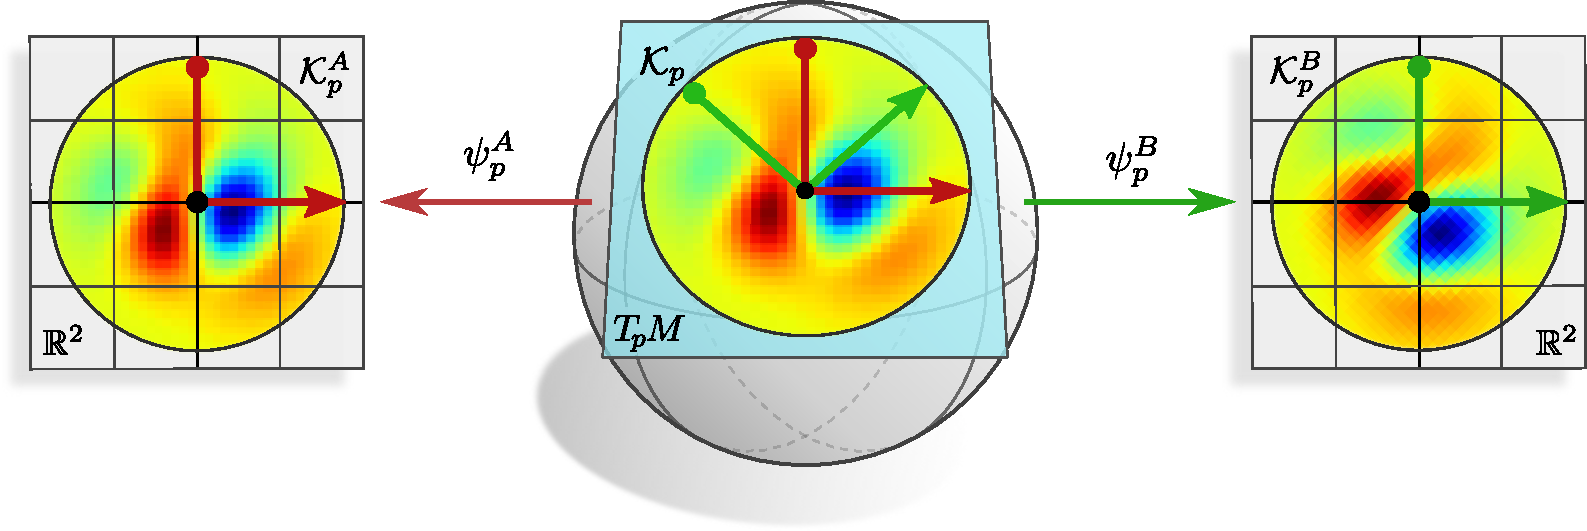
\includegraphics[width=.9\columnwidth]{figures/kernel_coordinatization.pdf}
	\caption{\small
		یک کرنل بدون مختصات $\Kp$ روی $\TpM$ و عبارات مختصاتی آن ${\Kp^X \!: \R^d \to \R^{\cout\times\cin}}$ نسبت به پیمانه‌های $\psi_p^X$ (فقط یکی از کانال‌های کرنل ${\cout \times \cin}$ نشان داده شده است).
		تبدیلات پیمانه‌ای که مختصات‌دهی‌های مختلف یک کرنل را به هم مرتبط می‌کنند، از قوانین تبدیل دامنه $\R^d$ و هم‌دامنه $\R^{\cout\times\cin}$ آن‌ها پیروی می‌کنند.
		بنابراین برای هر $\mathscr{v} \in \R^d$ به صورت
		$\Kp^B\big(g_p^{BA} \mathscr{v}\big) = \rhoout\big(g_p^{BA}\big) \:\Kp^A (\mathscr{v})\: \rhoin\big(g_p^{BA}\big)^{-1}$ داده می‌شوند.
		یک میدان کرنل $\K$ روی $M$ یک تخصیص هموار از کرنل‌ها بر روی فضاهای مماس است (تعریف~\ref{dfn:kernel_field_general}).
		\\
		توجه داشته باشید که ما در اینجا فرض می‌کنیم کرنل روی $\TpM$ داده شده است و سپس آن را نسبت به پیمانه‌های مختلف روی $\R^d$ بیان می‌کنیم.
		این از نظر مفهومی با وضعیت نشان داده شده در
		شکل‌های~\ref{fig:satellite}، \ref{fig:intro_kernel_alignment_trivial}، \ref{fig:gauge_trafos_feature_vector} و~\ref{fig:kernel_apx_sharing} متفاوت است،
		که در آنها فرض می‌کنیم یک کرنل الگو~$K$ روی $\R^d$ داده شده است و سپس $\Kp$ را روی $\TpM$ از طریق اشتراک‌گذاری وزن کانولوشنی نسبت به یک چارچوب مرجع تعریف می‌کنیم.
		برای حفظ استقلال از مختصات در طول فرآیند اشتراک‌گذاری وزن، کرنل مشترک باید تحت تبدیلات پیمانه \emph{پایا} (یا هموردا) باشد؛ به بخش~\ref{sec:gauge_conv} و پیوست~\ref{apx:coord_indep_weight_sharing} مراجعه کنید.
	}
	\label{fig:kernel_coordinatization}
\end{figure}

قانون تبدیل بین نمایش‌های مختصاتی $\Kp^A$ و $\Kp^B$ یک کرنل $\Kp$ روی $\TpM$ طبق معمول از قوانین تبدیل دامنه و هم‌دامنه آن‌ها پیروی می‌کند.
در دامنه $\R^d$ قانون تبدیل توسط $g_p^{BA}$ داده می‌شود، در حالی که قانون تبدیل $\R^{\cout\times\cin}$، همانند معادله~\eqref{eq:linear_op_trafo_law}، توسط یک ضرب همزمان از چپ با $\rhoout\big(g_p^{BA}\big)$ و از راست با $\rhoin\big(g_p^{BA}\big)^{-1}$ داده می‌شود.
بنابراین، دو مختصات‌دهی کرنل $\Kp$ برای هر $\mathscr{v} \in \R^d$ به صورت زیر با هم ارتباط دارند:
\begin{align}\label{eq:kernel_trafo_law}
	\Kp^B\big(g_p^{BA} \mathscr{v}\big)\ =\ 
	\rhoout\big(g_p^{BA}\big) \cdot\mkern1mu 
	\Kp^A (\mathscr{v})
	\mkern1mu\cdot \rhoin\big(g_p^{BA}\big)^{-1} \,,
\end{align}
که توسط نمودار جابجایی زیر به تصویر کشیده شده است:
\begin{equation}\label{cd:kernel_trafo_law}
	\qquad
	\begin{tikzcd}[column sep=70pt, row sep=32pt, font=\normalsize]
		\R^d
		\arrow[d, "g_p^{BA} \cdot\,"']
		\arrow[r, "\Kp^A"]
		&
		\R^{\cout\times\cin}
		\arrow[d, "\ \rhoout\big(g_p^{BA}\big) \; \scalebox{1.1}{$[\,\cdot\,]$} \; \rhoin\big(g_p^{BA}\big)^{-1}"]
		\\
		\R^d
		\arrow[r, "\Kp^B"']
		&
		\R^{\cout\times\cin}
	\end{tikzcd}
\end{equation}
همانند مثال‌های بخش~\ref{sec:pointwise_operations}، اصل کوواریانس تنها نیازمند یک رفتار تبدیل سازگار بین مختصات‌دهی‌های مختلف کرنل است اما محدودیتی بر خود کرنل اعمال نمی‌کند.
بنابراین می‌توان کرنل‌های $\Kp$ را برای هر $p\in M$ و یک پیمانه دلخواه در $p$ با یک کرنل ماتریس-مقدار نامحدود پارامتری کرد.
ما میدان‌های هموار چنین کرنل‌هایی را به عنوان میدان‌های کرنل نشان می‌دهیم که نقش عمده‌ای در تحلیل ما از هموردایی ایزومتری کانولوشن‌های $\GM$ در بخش~\ref{sec:isometry_intro} ایفا می‌کنند.

\paragraph{تبدیلات میدان کرنل مستقل از مختصات:}
با داشتن یک میدان کرنل هموار $\K$، می‌توانیم \emph{تبدیلات میدان کرنل} را تعریف کنیم، که شبیه به کانولوشن‌ها هستند اما از این جهت متفاوتند که ممکن است در هر موقعیت مکانی یک کرنل متفاوت اعمال کنند.
آنها یک میدان از بردارهای ویژگی خروجی $\fout(p)$ را با
انتگرال‌گیری از حاصلضرب کرنل مربوطه $\Kp$ و پس‌کِش انتقال‌دهنده $\Expspfin$ از $\fin$ روی $\TpM$ محاسبه می‌کنند، یعنی،
\begin{align}\label{eq:kft_coord_free}
	\fout(p)\ =\ 
	\int_{\TpM}
	\Kp(v) \,
	\Expspfin(v) \;
	dv \,.
\end{align}
برای بیان این تعریف بدون مختصات بر حسب مختصات، باید تمام کمیت‌ها را با عبارات مختصاتی‌شان جایگزین کرده و انتگرال‌گیری را از طریق پیمانه انتخاب‌شده از $\TpM$ به $\R^d$ منتقل کرد.
همانطور که در پیوست~\ref{apx:tangent_integral} توضیح داده شده است، عنصر حجم ریمانی مناسب (پایا نسبت به پیمانه) برای یک پیمانه $\psi_p^A$ به صورت زیر داده می‌شود:
\begin{align}
	\sqrt{|\eta_p^A|} \,\ dv^A ,
\end{align}
که در آن ضریب $\sqrt{|\eta_p^A|}$، تعریف شده در معادله~\eqref{eq:volume_element_def}، حجم (مثبت) پوشیده شده توسط چارچوب مرجع $[e_i^A]_{i=1}^d$ در~$p$ است.
بنابراین، عبارت مختصاتی تبدیل میدان کرنل به صورت زیر است:
\begin{align}\label{eq:kft_coord_expression}
	\fout^A(p)
	\ =&\ 
	\int_{\R^d}
	\Kp^A(v^A) \ 
	\big[\mkern-2mu \Expspfin\big]^A \mkern-1mu(v^A) \ 
	\sqrt{|\eta_p^A|}\ dv^A
	\,.
\end{align}
استقلال از مختصات تبدیل میدان کرنل با بیان آن نسبت به یک پیمانه جایگزین $\psi_p^B$ و نشان دادن اینکه میدان خروجی حاصل همانطور که انتظار می‌رود تبدیل می‌شود، تأیید می‌شود، که در واقع چنین است:
\begin{align}\label{eq:kft_coordinate_independence}
	\fout^B(p)\ 
	\overset{(1)}{=}&\ 
	\int_{\R^d}
	\Kp^B(v^B) \ 
	\big[\mkern-2mu \Expspfin\big]^B \mkern-2mu(v^B) \,\ 
	\sqrt{|\eta_p^B|}\ dv^B
	\notag \\ 
	\overset{(2)}{=}&\ 
	\int_{\R^d}
	\Big[ \rhoout\big(g_p^{BA}\big)\, \Kp^A\pig(\! \big(g_p^{BA}\big)^{-1} v^B \big)\!\pig)\, \rhoin\big(g_p^{BA}\big)^{-1} \Big] \,\ 
	\big[\mkern-1mu \Expspfin\big]^B \mkern-2mu(v^B) \,\ 
	\sqrt{|\eta_p^B|}\ dv^B
	\notag \\ 
	\overset{(3)}{=}&\ \ 
	\rhoout\big(g_p^{BA}\big)
	\int_{\R^d}
	\Kp^A(v^A) \,\ 
	\Big[ \rhoin\big(g_p^{BA}\big)^{-1} \big[\mkern-1mu \Expspfin\big]^B \mkern-2mu \big( g_p^{BA} v^A\big) \Big] \ 
	\sqrt{|\eta_p^A|}\ dv^A
	\notag \\ 
	\overset{(4)}{=}&\ \ 
	\rhoout\big(g_p^{BA}\big)
	\int_{\R^d}
	\Kp^A(v^A) \,\ 
	\big[\mkern-1mu \Expspfin\big]^A \mkern-1mu (v^A) \ 
	\sqrt{|\eta_p^A|}\ dv^A
	\notag \\ 
	\overset{(5)}{=}&\ \ 
	\rhoout\big(g_p^{BA}\big) \, \fout^A(p)
\end{align}
در اینجا ما از تعریف تبدیلات میدان کرنل و قانون تبدیل کرنل‌ها (معادله~\eqref{eq:kernel_trafo_law}) در دو مرحله اول استفاده کردیم.
مرحله سوم با بیرون کشیدن $\rhoout$ از انتگرال و جایگزینی $v^B$ با $v^A = \big(g_p^{BA}\big)^{-1} v^B$ به دست می‌آید، با استفاده از اینکه عنصر حجم $\sqrt{|\eta_p^B|}\ dv^B = \sqrt{|\eta_p^A|}\ dv^A$ به طور طراحی شده پایا نسبت به پیمانه است.
دو مرحله آخر با شناسایی قانون تبدیل پس‌کِش انتقال‌دهنده میدان ویژگی در معادله~\eqref{eq:trafo_law_transporter_pullback} و تعریف تبدیل میدان کرنل در پیمانه $\psi_p^A$ به دست می‌آیند.
توجه داشته باشید که استقلال از مختصات تبدیل میدان کرنل، صحت قانون تبدیل کرنل در معادله~\eqref{eq:kernel_trafo_law} را تأیید می‌کند.

یک تبدیل میدان کرنل تنها زمانی به خوبی تعریف می‌شود که انتگرال‌ها روی فضاهای مماس همگرا باشند، که به طور دقیق‌تر در بخش~\ref{sec:global_conv} و پیوست~\ref{apx:smoothness_kernel_field_trafo} مورد بحث قرار گرفته است.
قضیه~\ref{thm:existence_kernel_field_trafo_compact_kernels} ثابت می‌کند که یک تکیه‌گاه فشرده برای کرنل‌های $\Kp$ برای تضمین این خوش‌تعریفی کافی است.
این قضیه همچنین ثابت می‌کند که تبدیلات میدان کرنل که بر اساس میدان‌های کرنل هموار هستند، میدان‌های ویژگی ورودی هموار را به میدان‌های ویژگی خروجی هموار نگاشت می‌کنند.

\subsubsection{کانولوشن‌های \textit{\lr{GM}} و کرنل‌های \textit{\lr{G}}-راهبر}
\label{sec:gauge_conv}

آزادی تبدیلات میدان کرنل در اعمال یک کرنل متفاوت در هر مکان، به آنها اجازه تعمیم استنتاج آموخته‌شده را بر روی مکان‌های مختلف نمی‌دهد و بنابراین آنها را از نظر داده ناکارآمد می‌سازد.
بنابراین، معمولاً کانولوشن‌ها در نظر گرفته می‌شوند، که می‌توان آن‌ها را به عنوان آن دسته از تبدیلات میدان کرنل خاصی دید که بر اساس میدان‌های کرنل کانولوشنی هستند، یعنی میدان‌های کرنلی که توسط یک کرنل الگوی واحد و مشترک پارامتری شده‌اند.
همانند قبل، یک اشتراک‌گذاری وزن مستقل از مختصات نیازمند آن است که کرنل‌های الگو نسبت به پیمانه هموردا ($G$-راهبر) باشند.
این هموردایی پیمانه‌ای کرنل‌های الگو تضمین می‌کند که الگوهایی که در ژست‌های هندسی مختلف و مرتبط با $G$ ظاهر می‌شوند، تا یک تبدیل متناظر بردار ویژگی از طریق $\rhoout$ پاسخ یکسانی را برانگیزند.

\paragraph{اشتراک‌گذاری وزن کانولوشنی:}
فرض کنید $K: \R^d \to \R^{\cout\times\cin}$ یک کرنل الگو باشد که باید روی تمام فضاهای مماس به اشتراک گذاشته شود.
برای اینکه هیچ پیمانه خاصی را ترجیح ندهیم -- که با نیاز ما به استقلال از مختصات در تضاد است -- مجبوریم کرنل را با مختصات‌دهی‌ها در تمام پیمانه‌ها به طور همزمان به اشتراک بگذاریم.
به طور ساده‌انگارانه، این به نظر می‌رسد که پیشنهاد می‌کند کرنل الگو را با قرار دادن $\Kp^X = K$ برای هر نقطه $p\in M$ و هر پیمانه $\psi_p^X$ در~$p$ به اشتراک بگذاریم.
در حالی که چنین تعریفی از اشتراک‌گذاری کرنل معقول به نظر می‌رسد، از اصل ما برای اشتراک‌گذاری توابع الگوی محلی به معنای دقیق پیروی نمی‌کند:
به جای اشتراک‌گذاری مستقیم کرنل، مهم است که \emph{کل} عملیات محلی را به اشتراک بگذاریم ـ که در اینجا کل
تبدیل انتگرالی در معادله~\eqref{eq:kft_coord_expression} است.
از آنجایی که این عملیات بر حسب میدان کرنل $\K$ پارامتری می‌شود، این به طور غیرمستقیم منجر به اشتراک‌گذاری کرنل الگو می‌شود، با این حال، با نتیجه‌ای کمی متفاوت از اشتراک‌گذاری ساده‌انگارانه در نظر گرفته شده در بالا.

برای یافتن تعریف صحیح میدان‌های کرنل کانولوشنی $\GM$ طبق اصل ما برای اشتراک‌گذاری توابع الگوی محلی، ابتدا باید این عملیات محلی را شناسایی کنیم.
ما این کار را با انتزاع تبدیلات میدان کرنل (در مختصات) به عنوان مجموعه‌ای از عملگرهای انتگرالی محلی به شکل زیر انجام می‌دهیم:
\begin{align}\label{eq:local_integral_operator_general}
	\mathscr{I}_{\K,p}^A:\ 
	C^\infty \big(\R^d, \R^c\big) \to \R^c, \quad
	F \,\mapsto \int_{\R^d} \Kp^A(\mathscr{v})\, F(\mathscr{v})\, \sqrt{|\eta_p^A|}\ d\mathscr{v} \,,
\end{align}
که در آن $C^\infty \big(\R^d, \R^c\big)$ فضای نگاشت‌های هموار از $\R^d$ به $\R^c$ را نشان می‌دهد.
در کاربرد ما، این نگاشت‌های هموار صرفاً نمایش‌های میدان ویژگی محلی $[\Expspf]^A: \R^d \to \R^c$ هستند که از فضاهای مماس در~$p$ دیده می‌شوند و توسط تبدیل میدان کرنل به یک بردار ویژگی خروجی $\fout^A(p) = \mathscr{I}_{\K,p}^A \big([\Expspf]^A\big)$ در~$p$ نگاشته می‌شوند.
با توجه به کرنل الگوی ما $K: \R^d \to \R^{\cout\times\cin}$، ما یک الگوی عملگر انتگرالی متناظر را تعریف می‌کنیم:
\begin{align}\label{eq:local_integral_operator_template}
	\mathfrak{I}_K:\ 
	C^\infty \big(\R^d, \R^c\big) \to \R^c, \quad
	F \,\mapsto \int_{\R^d} K(\mathscr{v})\, F(\mathscr{v})\ d\mathscr{v} \,,
\end{align}
که نمایش میدان محلی $F$ را در کرنل الگو $K$ ضرب کرده و سپس حاصلضرب آنها را انتگرال می‌گیرد.
توجه داشته باشید که $\mathfrak{I}_K$ به عنوان یک تابع الگو لزوماً نسبت به انتخاب‌های خاص پیمانه‌ها بی‌تفاوت است و بنابراین شامل ضریب حجم چارچوب نمی‌شود.
یک طرح اشتراک‌گذاری وزن کانولوشنی مستقل از مختصات $\GM$ با الزام به اینکه این تابعک الگو با تمام عملگرهای انتگرالی منفرد در هر نقطه و در هر پیمانه موافق باشد، تحمیل می‌شود، یعنی:
\begin{align}\label{eq:weight_sharing_integral_operator}
	\mkern28mu
	\mathscr{I}_{\K,p}^X = \mathfrak{I}_K
	\quad \textup{برای \emph{هر} پیمانه}\ \ \big(U^X,\psi^X) \in \mathscr{A}^G\ \ \textup{با}\ \ p\in U^X \,,
\end{align}
که در آن $\mathscr{A}^G$ اطلس $G$ (ماکسیمال) متناظر با ساختار $G$ در نظر گرفته شده است؛ به معادله~\eqref{eq:G_atlas_dfn} مراجعه کنید.
این معادل اشتراک‌گذاری مستقیم کرنل الگوی محلی طبق زیر است:
\begin{align}\label{eq:weight_sharing_kernel}
	\Kp^X = \frac{K}{\sqrt{|\eta_p^X|}\,}
	\quad \textup{برای \emph{هر} پیمانه}\ \ \big(U^X,\psi^X) \in \mathscr{A}^G\ \ \textup{با}\ \ p\in U^X \,,
\end{align}
که در آن ضریب نرمال‌سازی «چگالی کرنل» را به اندازه حجم چارچوب مرجع $\sqrt{|\eta_p^X|}$ کاهش می‌دهد.
همانطور که در ادامه بحث می‌شود، این نرمال‌سازی برای هموردایی تحت گروه‌های تقارن غیر حافظ حجم مهم است.

ما میدان‌های کرنلی را که توسط یک کرنل مشترک $K$ طبق معادله~\eqref{eq:weight_sharing_kernel} پارامتری شده‌اند، به عنوان \emph{میدان‌های کرنل کانولوشنی} $\GM$ می‌نامیم.
الزام همزمان برای اشتراک‌گذاری وزن و استقلال از مختصات منجر به یک قید هموردایی بر روی کرنل‌های الگو می‌شود.
برای استخراج این قید، اشتراک‌گذاری کرنل در معادله~\eqref{eq:weight_sharing_kernel} را در قانون تبدیل کرنل در معادله~\eqref{eq:kernel_trafo_law} قرار می‌دهیم، که نتیجه می‌دهد:
\begin{align}
	\frac{1}{\sqrt{|\eta_p^B|\,}}\ K\big(g_p^{BA} \mathscr{v}\big)
	\ =\ 
	\frac{1}{\sqrt{|\eta_p^A|\,}}\ 
	\rhoout\big(g_p^{BA}\big) \cdot\mkern1mu 
	K(\mathscr{v})
	\mkern1mu\cdot \rhoin\big(g_p^{BA}\big)^{-1} \,.
\end{align}
از آنجایی که حجم‌های چارچوب‌های مرجع مختلف با
$\sqrt{|\eta_p^A|} = \big|\mkern-2mu \det(g_p^{BA})\big|\, \sqrt{|\eta_p^B|}$
مرتبط هستند و از آنجایی که قانون تبدیل باید برای پیمانه‌های دلخواه مرتبط با $G$ برقرار باشد، این قید \emph{$G$-راهبری} را ایجاب می‌کند%
\footnote{
	برخلاف کارهای قبلی~\cite{3d_steerableCNNs,Weiler2019_E2CNN,gaugeIco2019,kicanaoglu2019gaugeSphere,deHaan2020meshCNNs}، این قید شامل ضریب $\detg$ است.
	این ضریب در آن کارها ظاهر نشد زیرا همه آنها گروه‌های ساختاری متعامد $\OO{d}$ (یا زیرگروه‌های آن) را در نظر گرفته بودند که برای آنها ضریب دترمینان صفر می‌شود.
}
\begin{align}\label{eq:kernel_constraint}
	K(g\mkern1.5mu \mathscr{v})\ = \ \frac{1}{\detg}\, \rhoout(g) \cdot K(\mathscr{v}) \cdot \rhoin(g)^{-1}
	\qquad \forall\ \ \mathscr{v} \in \R^d,\ \ g\in G \,.
\end{align}
بر روی کرنل‌های الگو.
همانطور که توسط لانگ و همکاران~\cite{lang2020WignerEckart} ثابت شده است، این قید نیازمند آن است که کرنلهای الگو \emph{عملگرهای نمایش}~\cite{jeevanjee2011reprOp} باشند (تعمیمهایی از عملگرهای تانسوری کروی در مکانیک کوانتومی).
از نظر نموداری، یک کرنل $G$-راهبر $K$ باید جابجایی زیر را برآورده کند:
\begin{equation}\label{cd:kernel_steerability}
	\qquad\qquad
	\begin{tikzcd}[column sep=70pt, row sep=35pt, font=\normalsize]
		\R^d
		\arrow[d, "g\mkern2mu \cdot\,"']
		\arrow[r, "K"]
		&
		\R^{\cout\times\cin}
		\arrow[d, "\ \scalebox{.96}{$\displaystyle \frac{1}{\detg}$}\, \rhoout(g) \; \scalebox{1.1}{$[\,\cdot\,]$} \; \rhoin(g)^{-1}"]
		\\
		\R^d
		\arrow[r, "K"']
		&
		\R^{\cout\times\cin}
	\end{tikzcd}
\end{equation}
برای هر $g\in G$.
توجه داشته باشید که ضریب دترمینان معکوس $\detg$ در قانون تبدیل کرنل باعث می‌شود که آن مانند یک \emph{$(-1)$-چگالی ماتریس-مقدار} تبدیل شود؛ برای جزئیات بیشتر به جدول~\ref{tab:density_factors} مراجعه کنید.
به طور شهودی، کرنل‌های $G$-راهبر دقیقاً آن کرنل‌هایی هستند که می‌توانند نسبت به چارچوب‌های مرجع دلخواه مرتبط با $G$ به اشتراک گذاشته شوند بدون اینکه انتخاب خاص پیمانه بر نتیجه تأثیر بگذارد.%
\footnote{
	قید $G$-راهبری را می‌توان به صورت
	${K(\mathscr{v}) = \detg^{\minus1} \rhoout(g) \mkern-1mu\cdot\mkern-1.5mu K(g^{\minus1}\mathscr{v}) \mkern-1mu\cdot\mkern-1.5mu \rhoin(g)^{\minus1}}$
	$\mkern8mu \forall\ \mathscr{v} \in \R^d,\ g\in G$
	بازنویسی کرد، که تأکید می‌کند کرنل‌های $G$-راهبر \emph{پایاها} تحت عمل پیمانه در سمت راست هستند.
	یک کرنل $G$-راهبر، با پایا بودن تحت تبدیلات پیمانه، منجر به همان کرنل بدون مختصات $\Kp$ در $p$ می‌شود، زمانی که نسبت به هر چارچوب مرجعی در~$\GpM$ به اشتراک گذاشته شود.
}
بنابراین، ابهام هم‌ترازی کرنل‌ها ـ که انگیزه اصلی این کار بود -- با اشتراک‌گذاری وزن اضافی بر روی تمام چارچوب‌های مرجع معادل (تمام پیمانه‌ها) در ساختار $G$ در نظر گرفته شده~$\GM$ حل می‌شود.

\begin{table}[H]
	\centering
	\setlength\aboverulesep{0pt}
	\setlength\belowrulesep{0pt}
	\renewcommand{\arraystretch}{1.8}
	\setlength{\tabcolsep}{2.4ex}
	\scalebox{.95}{
		\begin{tabular}{l|ccccccc}
			شیء & $\Kp^X$ & $K$ & $\big[\mkern-2mu\Expspf\big]^{\mkern-2muX}\mkern-2mu$ و $F$ & $\sqrt{|\eta^X|}$ & $dv^X\!$ و $d\mathscr{v}$ \\
			\midrule
			چگالی $s$ & $0$ & $-1$ & $0$ & $-1$ & $1$
		\end{tabular}
	}
	\vspace*{2ex}
	\caption{
		مروری بر توان‌های چگالی $s$ برای اشیاء مختلف درگیر در تبدیلات میدان کرنل عمومی و کانولوشن‌های $\GM$.
		عبارت مختصاتی یک $s$-چگالی با ضریب $\detg^s$ تبدیل می‌شود وقتی مختصات از طریق $g\in G$ تبدیل شوند.
		یک کرنل ماتریس-مقدار عمومی $\Kp^X$ طبق معادله~\eqref{eq:kernel_trafo_law} یک $0$-چگالی است.
		همین امر برای میدان‌های ویژگی و پس‌کِش‌های آنها نیز صادق است که قوانین تبدیل آنها در معادلات~\eqref{eq:gauge_trafo_features} و~\eqref{eq:trafo_law_transporter_pullback} داده شده است.
		کل انتگرال‌ده $\Kp^X(v^X) [\Expspf]^{\mkern-1muX}(v^X) \sqrt{|\eta^X|}\, dv^X$ از یک تبدیل میدان کرنل عمومی در معادله~\eqref{eq:kft_coord_expression} نیز یک $0$-چگالی دیده می‌شود -- توجه داشته باشید که این برای استقلال آن از مختصات، همانطور که در معادله~\eqref{eq:kft_coordinate_independence} نشان داده شده، ضروری است.
		از آنجایی که الگوی عملگر انتگرالی $\mathfrak{I}_K$ در معادله~\eqref{eq:local_integral_operator_template} نسبت به هر انتخاب پیمانه بی‌تفاوت است، شامل ضریب حجم چارچوب $\sqrt{|\eta^X|}$ نمی‌شود.
		از آنجایی که با این وجود باید مانند عملگرهای انتگرالی $\mathscr{I}_{\K,p}^X$ که زیربنای تبدیلات میدان کرنل هستند رفتار کند، کل انتگرال‌ده $K(\mathscr{v}) F(\mathscr{v})\, d\mathscr{v}$ از $\mathfrak{I}_K(F)$ ملزم به بودن یک $0$-چگالی است.
		این امر مستلزم آن است که خود کرنل‌های الگوی مشترک $K$ مانند $(-1)$-چگالی‌ها تبدیل شوند، که در قید $G$-راهبری در معادله~\eqref{eq:kernel_constraint} منعکس شده است.
		توجه داشته باشید که این قانون تبدیل کرنل‌های الگو برای هموردایی $G$ محلی کانولوشن‌های $\GM$ اکیداً ضروری است اگر ویژگی‌های خروجی باید مانند چگالی‌هایی با وزن $0$ تبدیل شوند؛ به معادله~\eqref{eq:active_local_gauge_trafo} مراجعه کنید.
		برای دیدگاهی جایگزین، خواننده علاقه‌مند را به نتیجه ۱ در~\cite{bekkers2020bspline} ارجاع می‌دهیم، جایی که ضریب دترمینان از اندازه‌های هار روی گروه‌های لی استخراج می‌شود.
	}
	\label{tab:density_factors}
\end{table}

قبل از پرداختن به کانولوشن‌های $\GM$، در مورد فضای کرنل‌های $G$-راهبر توضیح می‌دهیم.
توجه داشته باشید که مجموعه
\begin{align}\label{eq:unconstrained_kernel_space}
	\mathscr{K}\ :=\ \pig\{ K\!: \R^d \to \R^{\cout\times\cin} \pig\} \,.
\end{align}
کرنل‌های عمومی، یعنی نه لزوماً هموردا، با مجهز شدن به جمع و ضرب اسکالر استاندارد روی $\R^{\cout\times\cin}$ یک فضای برداری تشکیل می‌دهد.
از آنجایی که قید $G$-راهبری در معادله~\eqref{eq:kernel_constraint} خطی است، فضای کرنل را به یک \emph{زیرفضای خطی} محدود می‌کند:
\begin{align}\label{eq:G-steerable_kernel_space}
	\KG\, :=\ \Big\{ K\!: \R^d \to \R^{\cout\times\cin} \,\Big|\,
	K(g\mkern1mu \mathscr{v}) = \frac{1}{\detg}\, \rhoout(g) \mkern-1.5mu\cdot\mkern-1.5mu K(\mathscr{v}) \mkern-1.5mu\cdot\mkern-1.5mu \rhoin(g)^{-1} \ \ \ \forall\,\ \mathscr{v}\in \R^d,\,\ g\in G \Big\} \,.
\end{align}
بنابراین می‌توان برای یک پایه از کرنل‌های $G$-راهبر راه‌حلی یافت که کانولوشن $\GM$ را می‌توان بر حسب آن پارامتری کرد.
در حالی که این فضا در تئوری معمولاً بی‌نهایت-بعدی است، در عمل اغلب گسسته می‌شود، به طوری که در نهایت با یک پایه متناهی $\{K_1,\dots,K_N\}$ از کرنل‌های $G$-راهبر مواجه می‌شویم.
سپس یک مجموعه از وزن‌های با مقادیر حقیقی $\{w_1,\dots,w_N\}$ که $w_i\in\R$ هستند و در طول فرآیند آموزش بهینه‌سازی می‌شوند، کانولوشن را با $K = \sum_{i=1}^N w_i K_i$ پارامتری می‌کنند.
توجه داشته باشید که ابعاد کاهش‌یافته (زیر)فضای کرنل‌های $G$-راهبر به معنای بهبود کارایی پارامتر در مقایسه با کانولوشن‌های معمولی است.

بخش~\ref{sec:mobius_kernel_spaces} به بحث در مورد راه‌حل‌های تحلیلی نمونه‌ای از فضاهای کرنل هموردای بازتابی برای نمایش‌های گروهی مختلف گروه بازتاب~$\Flip$ می‌پردازد.
کرنل‌های حاصل که با انواع مختلفی از تقارن‌های بازتابی مشخص می‌شوند، در جدول~\ref{tab:reflection_steerable_kernels} به تصویر کشیده شده‌اند.

مثال‌های بیشتری را می‌توان در ادبیات مربوط به شبکه‌های عصبی کانولوشنی راهبر یافت:
یک راه‌حل تحلیلی برای قید فضای کرنل برای گروه ساختاری متعامد خاص $\SO3$ در سه بعد و نمایش‌های تحویل‌ناپذیر آن توسط توماس و همکاران~\cite{3d_steerableCNNs} ارائه شد.
وایلر و کوهن~\cite{Weiler2019_E2CNN} این رویکرد را برای پوشش نمایش‌های گروهی دلخواه تعمیم دادند و قید فضای کرنل را برای هر نمایشی از $\OO2$ و تمام زیرگروه‌های آن $G\leq\OO2$ حل کردند
-- یک پیاده‌سازی در \url{https://quva-lab.github.io/e2cnn/api/e2cnn.kernels.html} موجود است.
برای گروه‌های ساختاری متناهی، قید را می‌توان به صورت عددی نیز حل کرد، همانطور که توسط کوهن و ولینگ~\cite{Cohen2017-STEER} توضیح داده شده است.
یک استراتژی راه‌حل کلی‌تر، که برای گروه‌های ساختاری فشرده دلخواه~$G$ (و بنابراین همه موارد ذکر شده در بالا) کاربرد دارد، توسط لانگ و کورنبلیث~\cite{lang2020WignerEckart} پیشنهاد شد.
این راه‌حل قضیه کلاسیک \emph{ویگنر-اکارت}~\cite{agrawalla1980WignerEckart,jeevanjee2011reprOp,wigner1931gruppentheorie,wigner1993matrices} را به یک قضیه ویگنر-اکارت برای کرنل‌های $G$-راهبر تعمیم می‌دهد، که کرنل‌ها را بر حسب توابع پایه هارمونیک، ضرایب کلبش-گوردان و اندومورفیسم‌های نمایش‌ها (عناصر ماتریسی کاهش‌یافته تعمیم‌یافته) بیان می‌کند.
ما برای مروری دقیق‌تر بر کارهای قبلی و مرتبط با کرنل‌های راهبر به لانگ و کورنبلیث~\cite{lang2020WignerEckart} ارجاع می‌دهیم.

\paragraph{کانولوشن‌های مستقل از مختصات \textit{\lr{GM}}:}

با داشتن یک کرنل الگوی $G$-راهبر $K\in\KG$، کانولوشن $\GM$~$K\star$ با این کرنل به عنوان تبدیل میدان کرنل با میدان کرنل کانولوشنی $\GM$ متناظر تعریف می‌شود، که برای هر نقطه $p\in M$ و هر پیمانه $\psi_p^X$ در $\Kp^X = K / \sqrt{|\eta^X|}$ صدق می‌کند.
با قرار دادن میدان کرنل کانولوشنی $\GM$ در معادله~\eqref{eq:kft_coord_expression}، یعنی تبدیل میدان کرنل، عبارت مختصاتی کانولوشن $\GM$ به صورت زیر ساده می‌شود:
\begin{align}\label{eq:gauge_conv_coord_expression}
	\fout^A(p)
	\ =\ 
	\big[ K \star \fin \big]^A(p)
	\ :=&\,\ 
	\int_{\R^d} \!
	K(\mathscr{v}) \,
	\big[\mkern-2mu \Expspfin\big]^{\mkern-2mu A} \mkern-1mu(\mathscr{v})
	\; d\mathscr{v}
	\ \ =\,\ \mathfrak{I}_K \big( [\Expspfin]^A \big)
	\,.
\end{align}
بنابراین، این به سادگی با تطبیق پس‌کِش انتقال‌دهنده $[\Expspfin]^A$ از میدان ویژگی در یک \emph{پیمانه دلخواه انتخاب شده} $\psi_p^A$ با کرنل کانولوشن \emph{مستقل از پیمانه}~$K$ به دست می‌آید.
بنابراین کانولوشن‌های مستقل از مختصات $\GM$ به راحتی با
۱) انتخاب چارچوب‌های مرجع دلخواه،
۲) پس‌کِش (و انتقال) میدان‌های ویژگی به مختصات‌دهی‌های فضای مماس و
۳) انقباض آنها در آنجا با یک کرنل $G$-راهبر (قابل آموزش) پیاده‌سازی می‌شوند.

کانولوشن‌های $\GM$ چندین ویژگی تقارنی مرتبط را از خود نشان می‌دهند:
\begin{itemize}[leftmargin=13em]
	\item[\it استقلال از مختصات:]
	به عنوان موارد خاصی از تبدیلات میدان کرنل، کانولوشن‌های $\GM$ به طور (غیرفعال) مستقل از مختصات هستند، یعنی معادله~\eqref{eq:kft_coordinate_independence} در مورد آنها صدق می‌کند.
	\item[\it هموردایی ایزومتری سراسری:]
	آنها تحت عمل \emph{فعال} و \emph{سراسری} ایزومتری‌های حافظ ساختار $G$ در $\IsomGM$ بر روی میدان‌های ویژگی هموردا هستند.
	بخش‌های~\ref{sec:gauge_conv_isom_equiv} و به ویژه~\ref{sec:isometry_intro} این ویژگی را به تفصیل مورد بحث قرار می‌دهند.
	\item[\it هموردایی $G$ محلی:]
	الگوی عملگر انتگرالی $\mathfrak{I}_K$ به دلیل $G$-راهبری~$K$ خود $G$-هموردا است.
	بنابراین، هر تبدیل $G$ یک نمایش میدان ویژگی محلی روی $\R^d$ منجر به تبدیل متناظر بردار ویژگی حاصل خواهد شد؛ به شکل~\ref{fig:active_TpM_equivariance} مراجعه کنید.
	بنابراین، تبدیلات $G$ مستقل الگوهایی که در نقاط مختلف $p_i\in M$ متمرکز شده‌اند، منجر به تبدیلات ویژگی خروجی مستقل در این نقاط می‌شوند (این \emph{فقط} در این نقاط برقرار است و نیازمند کرنل‌هایی با تکیه‌گاه فشرده است که کل \emph{میدان دید} آنها طبق تبدیل $G$ تبدیل شود).
\end{itemize}

\begin{figure}[H]
	\centering
	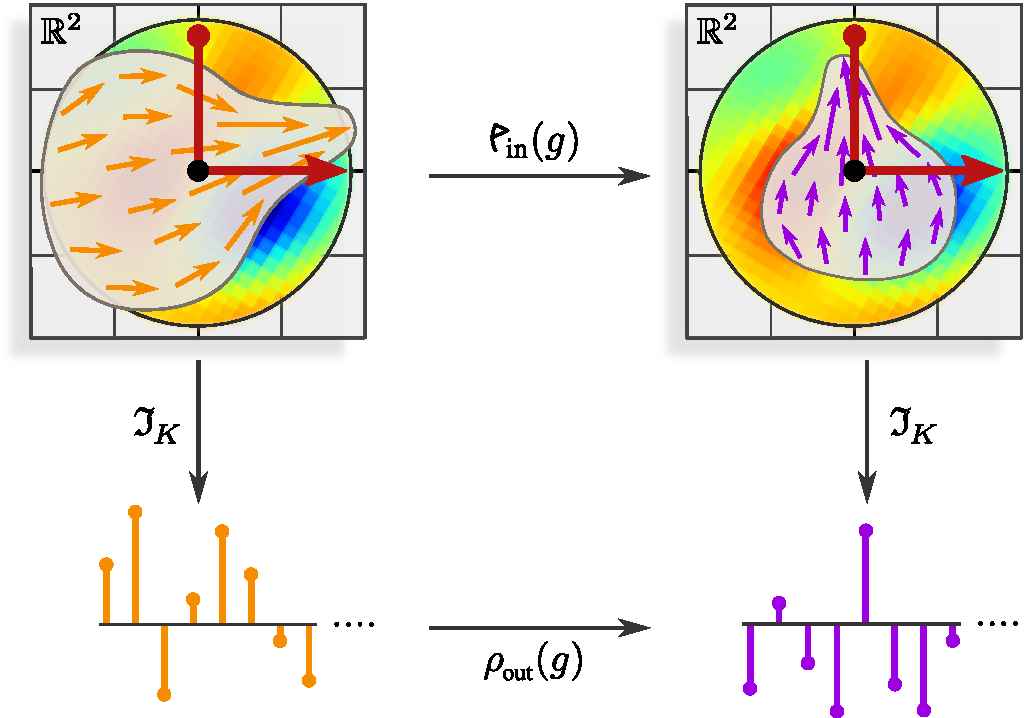
\includegraphics[width=.65\columnwidth]{figures/active_TpM_equivariance.pdf}
	\vspace*{1ex}
	\caption{\small
		هموردایی $G$ محلی الگوی عملگر انتگرالی مشترک $\mathfrak{I}_K$ که زیربنای یک کانولوشن $\GM$~$K\star$ است.
		یک تبدیل $G$ فعال $\mathfrakb_{\mkern-5mu\textup{\lr{in}}}(g)$ از یک نمایش میدان محلی روی $\R^d$ بردارهای ویژگی را از $g^{-1}\mathscr{v}$ به~$\mathscr{v}$ منتقل می‌کند و آنها را علاوه بر این از طریق $\rhoin(g)$ تبدیل می‌کند.
		در حالی که اولی ویژگی‌ها را به صورت فضایی جابجا می‌کند، دومی ضرایب عددی آنها را تبدیل می‌کند (که در شکل به صورت چرخش و مقیاس‌بندی بردارهای (مماس) منفرد به تصویر کشیده شده است).
		اعمال $\mathfrak{I}_K$ به هر دو ورودی منجر به بردارهای ویژگی خروجی متفاوتی می‌شود.
		با این حال، به دلیل هموردایی $G$ از $\mathfrak{I}_K$، تضمین می‌شود که پاسخ‌ها با $\rhoout(g)$ مرتبط هستند؛ به معادله~\eqref{eq:active_local_gauge_trafo} مراجعه کنید.
		بنابراین، یک تبدیل $G$ فعال از یک میدان ورودی منجر به یک تبدیل $G$ فعال متناظر از بردار ویژگی خروجی می‌شود.
		توجه داشته باشید که هموردایی $G$ از $\mathfrak{I}_K$ یک نتیجه مستقیم از $G$-راهبری $K$ است.
		\\\protect\rule{0ex}{0.5ex}
	}
	\label{fig:active_TpM_equivariance}
\end{figure}

برای دقیق‌تر کردن نکته آخر، ما تبدیلات $G$ فعال نمایش‌های میدان ویژگی محلی را در $C^\infty(\R^d,\R^c)$ به صورت زیر تعریف می‌کنیم%
\footnote{
	${\mathfrakb = \Res_G^{\R^d\mkern-1mu\rtimes G}\Ind_G^{\R^d\mkern-1mu\rtimes G}\!\rho}$ به طور رسمی با القای نمایش $G$ $\rho$ به یک نمایش ${(\R^d\mkern-4mu\rtimes\mkern-2muG)}$ ${ \Ind_G^{\R^d\mkern-1mu\rtimes G}\!\rho}$، و سپس محدود کردن آن به $G$ داده می‌شود.
	یک توضیح شهودی از نمایش‌های القایی و محدود شده را می‌توان در پیوست B از~\cite{Weiler2019_E2CNN} یافت در حالی که \cite{gallier2019harmonicRepr} این موضوع را به طور رسمی‌تر بررسی می‌کند.
}
\begin{align}\label{eq:local_field_G_trafo}
	\mathfrakb_{\mkern-5mu\textup{\lr{in}}}:\ 
	G \times C^\infty(\R^d,\R^c) \to C^\infty(\R^d,\R^c) \,, \quad
	F \,\mapsto\, \mathfrakb_{\mkern-5mu\textup{\lr{in}}}(g)F \,:=\, \rhoin(g) \circ F \circ g^{-1} \,,
\end{align}
که در آن فرض می‌کنیم $F$ از نوع $\rhoin$ است.
به طور شهودی، $\mathfrakb_{\mkern-5mu\textup{\lr{in}}}$ با انتقال فعال بردارهای ویژگی $F(g^{-1}\mathscr{v}) \in \R^c$ از $g^{-1}\mathscr{v}$ به $\mathscr{v}$ و تبدیل آنها با $\rhoin(g)$ بر روی میدان‌های $F$ عمل می‌کند
ـ این تعریف «معمولی» تبدیلات فعال میدان‌های ویژگی~$F$ بر روی فضاهای اقلیدسی~$\R^d$ است.
هموردایی $G$ ادعا شده برای $\mathfrak{I}_K$ به راحتی با اعمال آن به یک ورودی تبدیل شده، و سپس جایگزینی و استفاده از $G$-راهبری~$K$ دیده می‌شود:
\begin{align}\label{eq:active_local_gauge_trafo}
	\mathfrak{I}_K \big( \mathfrakb_{\mkern-5mu\textup{in}}(g) F \big)
	&= \mathfrak{I}_K \big( \rhoin(g) \circ F \circ g^{-1} \big)
	&& \big( \text{\small تعریف $\mathfrakb_{\mkern-5mu\textup{in}}$، معادله~\eqref{eq:local_field_G_trafo} } \big) \notag\\
	&= \int_{\R^d} K(\mathscr{v})\; \rhoin(g)\, F\big(g^{-1}\mathscr{v})\ d\mathscr{v}
	&& \big( \text{\small تعریف $\mathfrak{I}_K$، معادله~\eqref{eq:local_integral_operator_template} } \big) \notag\\
	&= \int_{\R^d} K(g\mkern1mu\tilde{\mathscr{v}})\; \rhoin(g)\, F\big(\tilde{\mathscr{v}})\; \detg \ d\tilde{\mathscr{v}}
	&& \big( \text{\small جایگزینی $\tilde{\mathscr{v}} = g^{-1} \mathscr{v}$ } \big) \notag\\
	&= \int_{\R^d} \rhoout(g)\, K(\tilde{\mathscr{v}})\; F\big(\tilde{\mathscr{v}})\ d\tilde{\mathscr{v}}
	&& \big( \text{\small $G$-راهبری $K$، معادله~\eqref{eq:kernel_constraint} } \big) \notag\\
	&= \rhoout(g)\; \mathfrak{I}_K(F)
	&& \big( \text{\small تعریف $\mathfrak{I}_K$، معادله~\eqref{eq:local_integral_operator_template} } \big)
\end{align}
بنابراین، یک تبدیل فعال یک نمایش میدان ویژگی محلی $F$ روی یک مختصات‌دهی فضای مماس با~$\mathfrakb_{\mkern-5mu\textup{\lr{in}}}(g)$ تضمین می‌کند که منجر به تبدیل بردار ویژگی خروجی حاصل با~$\rhoout(g)$ می‌شود.
به عبارت دیگر، ویژگی‌هایی که در ژست‌های هندسی مختلف مرتبط با $G$ ظاهر می‌شوند، تا یک تبدیل از طریق~$\rhoout$ پاسخ یکسانی را برمی‌انگیزند.
این به طور خلاصه در قالب یک نمودار جابجایی به صورت زیر است:
\begin{equation}\label{cd:active_G_equivariance}
	\begin{tikzcd}[column sep=56pt, row sep=34pt, font=\normalsize]
		C^\infty(\R^d,\R^{\cin})
		\arrow[d, "\mathfrak{I}_K\,"']
		\arrow[r, "\mathfrakb_{\mkern-5mu\textup{\lr{in}}}(g)"]
		&
		C^\infty(\R^d,\R^{\cin})
		\arrow[d, "\ \mathfrak{I}_K"]
		\\
		\R^{\cout}
		\arrow[r, "\rhoout(g)"']
		&
		\R^{\cout}
	\end{tikzcd}
\end{equation}
شکل~\ref{fig:active_TpM_equivariance} یک تفسیر بصری از این ویژگی هموردایی $\mathfrak{I}_K$ ارائه می‌دهد.

توجه داشته باشید که هموردایی تحت تبدیلات $G$ محلی در معادله~\eqref{eq:active_local_gauge_trafo} دقیقاً به قید $G$-راهبری همانطور که در معادله~\eqref{eq:kernel_constraint} است، یعنی به طور خاص، \emph{با} ضریب دترمینان $\detg^{-1}$ که باعث می‌شود کرنل مانند یک $(-1)$-چگالی تبدیل شود، نیاز دارد.
این ضریب به تعریف ما از اشتراک‌گذاری وزن کانولوشنی در معادله~\eqref{eq:weight_sharing_kernel} \emph{با} نرمال‌سازی با حجم‌های چارچوب مرجع $\sqrt{|\eta_p^X|}$ برمی‌گردد.
بنابراین، اشتراک‌گذاری وزن ساده‌انگارانه‌ای که در ابتدای این بخش ذکر شد، به رفتار تبدیل مطلوب منجر نمی‌شد.
به عبارت دیگر: هر دو نسخه ساده‌انگارانه و نرمال‌شده اشتراک‌گذاری کرنل مستقل از مختصات هستند و بنابراین هر دو تحت تبدیلات پیمانه غیرفعال ـ به ویژه آنهایی که حجم چارچوب را تغییر می‌دهند ـ به طور سازگار رفتار می‌کنند.
با این حال، در مورد اشتراک‌گذاری کرنل ساده‌انگارانه، این امر توسط پایایی عنصر حجم ریمانی $\sqrt{|\eta_p^A|}\ dv^A = \sqrt{|\eta_p^B|}\ dv^B$ مراقبت می‌شود.
با \emph{حذف} این ضریب در اشتراک‌گذاری وزن نرمال‌شده، سازگاری رفتار تبدیل دیگر توسط خود اندازه انتگرال‌گیری تضمین نمی‌شود ـ که مستلزم آن است که خود کرنل‌های $G$-راهبر تغییرات حجم را از طریق ضریب دترمینان توضیح دهند.
فقط دومی به تبدیلات فعال تعمیم می‌یابد، جایی که فقط میدان ویژگی تبدیل می‌شود، در حالی که اندازه انتگرال‌گیری پایا می‌ماند.

از آنجایی که تعریف ما از کانولوشن‌های $\GM$ امکان خمینه‌های ریمانی، ساختارهای G و انواع میدان دلخواه را فراهم می‌کند، بسیار عمومی است و طیف گسترده‌ای از کارهای مرتبط را پوشش می‌دهد.
ما این ادعا را در بخش~\ref{part:literature_review} اثبات می‌کنیم، جایی که بسیاری از \cnn{}ها را روی فضاهای آفین اقلیدسی $\Euc_d$، کره $S^2$ و خمینه‌ها یا مش‌های عمومی به عنوان نمونه‌های خاصی از معادله~\eqref{eq:gauge_conv_coord_expression} توضیح می‌دهیم.
برای یک نمای کلی و طبقه‌بندی این مدل‌ها، به جدول~\ref{tab:network_instantiations} مراجعه کنید.